\section{Automated Testing-as-a-Service (TaaS)}


\section{Layered Symbolic Execution}


\subsubsection{Case Study \#1: UNIX Utilities}
\label{sec:coreutils}

\topic{\klee is an excellent tool for testing command-line programs, in particular \unix utilities.}  It does not tackle more complex systems, like the ones in Table~\ref{table:tested}, mainly due to path explosion (since \klee is a single-node engine) and insufficient environment support.  We cannot compare \cnine to \klee on parallel and distributed systems, but we can compare on the Coreutils suite of \unix utilities~\cite{coreutils}.

We run \klee on each of the 96 utilities for 10 minutes, and then  run a 12-worker \cnine on each utility for 10 minutes. Fig.~\ref{fig:coreutils-cov} reports the average coverage increase obtained with \cnine over 7 trials, using \klee's 7-trial average results as a baseline; the experiment totals $2 \times 7 \times 96 \times 10 = 13,440$ minutes $>$ 9 days.  The increase in coverage is measured as {\em additional} lines of code covered, expressed as a percentage of program size (i.e., we do not report it as a percentage of the baseline, which would be a higher number).

\topic{\cnine covers up to an additional $40\%$ of the target programs, with an average of $13\%$ additional code covered across all Coreutils.}  In general, improving coverage becomes exponentially harder as the base coverage increases, and this effect is visible in the results: a $12\times$ increase in hardware resources does not bring about a $12\times$ increase in coverage.  Our results show that \cnine allows ``throwing hardware'' at the automated testing problem, picking up where \klee left off.  In three cases, \cnine achieved $100\%$ coverage in 10 minutes on real-world code.  This experiment does not aim to show that \cnine is a ``better'' symbolic execution engine than \klee---after all, \cnine is based on \klee---but rather that \cnine-style parallelization can make existing symbolic execution engines more powerful.

The way we compute coverage is different from~\cite{klee}---whereas \klee was conceived as an automated {\em test generator}, \cnine is meant to {\em directly test} software. Thus, we measure the number of lines of code tested by \cnine, whereas \cite{klee} reports numbers obtained by running the concrete test cases generated by \klee.  Our method yields more-conservative numbers because a test generated by \klee at the end of an incomplete path (e.g., that terminated due to an environment failure) may execute further than the termination point when run concretely.

\begin{figure}[h!]
  \centering
  \label{fig:coreutils-final-cov}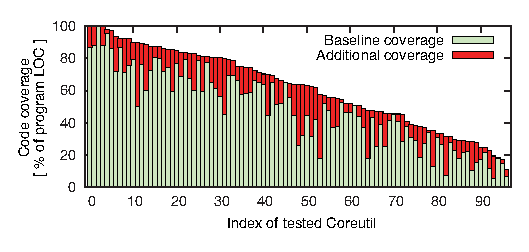
\epsfig{file=figures/evaluation/coreutils-cov-edited.eps, width=3.2in} \\
  \label{fig:coreutils-delta-cov}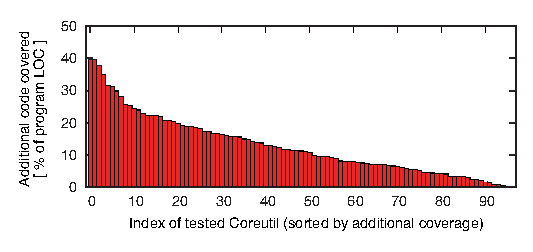
\epsfig{file=figures/evaluation/coreutils-delta-cov-edited.eps, width=3.2in}
  \caption{\cnine coverage improvements on the 96 Coreutils (1-worker \cnine vs. 12-worker \cnine).}
  \label{fig:coreutils-cov}
\end{figure}


%%% Local Variables: 
%%% mode: latex
%%% eval: (visual-line-mode)
%%% fill-column: 1000000
%%% TeX-master: "main"
%%% End:
